\documentclass[10pt]{article}
\usepackage[margin=0.82in]{geometry}
\usepackage{amsmath,amssymb,booktabs,graphicx,array,tabularx,longtable,float,microtype,enumitem,xcolor,hyperref,fancyhdr,calc,listings}
\usepackage[T1]{fontenc}
\usepackage{lmodern}
\hypersetup{colorlinks=true,linkcolor=blue!45!black,citecolor=blue!45!black,urlcolor=blue!45!black,pdftitle={MMALS-CAL v0.3.2},pdfauthor={Guillaume Harbonnier}}
\pagestyle{fancy}\fancyhf{}\lhead{MMALS-CAL v0.3.2}\rhead{Harbonnier}\cfoot{\thepage}
\newcommand{\mmalscal}{\textsc{MMALS-CAL}}
\newcommand{\action}{\texttt{ACTION}}
\newcommand{\nodecision}{\texttt{NO\_DECISION}}

\providecommand{\tightlist}{\setlength{\itemsep}{0pt}\setlength{\parskip}{0pt}}
\DeclareUnicodeCharacter{2192}{\ensuremath{\rightarrow}}
\DeclareUnicodeCharacter{2193}{\ensuremath{\downarrow}}
\lstset{
  basicstyle=\ttfamily\small,
  breaklines=true,
  frame=single,
  columns=fullflexible,
  keepspaces=true,
  literate={→}{{$\rightarrow$}}1 {↓}{{$\downarrow$}}1 {“}{{``}}1 {”}{{''}}1 {’}{{'}}1
}
\title{\bfseries MMALS-CAL: Regime-Aware Conformal Evidence Verification for Continual-Learning Systems\\\large Version 0.3.2 - Offline Cross-Benchmark Evidence Synthesis}
\author{Guillaume Harbonnier\\Independent MMALS Research Program}
\date{June 2026}
\begin{document}
\maketitle

\begin{abstract}
Continual-learning evaluations emphasize accuracy, retention, and forgetting, but a deployed system must answer an additional question: is its current prediction supported by evidence that is valid for the present regime and sufficiently precise to justify action? We introduce \mmalscal{}, a standalone companion verification layer within the MMALS program. It separates predictive competence, context recognition, marginal coverage, prediction-set compactness, and operational actionability. We execute a harmonized offline replay over seven final-checkpoint selected-policy traces comprising 250,000 observations, five seeds per benchmark, and five calibration strategies. Fresh oracle-regime calibration reaches aggregate coverage between 0.8889 and 0.9062 for a 0.90 target, while singleton action rates range from 0.15\% on CORe50 to 92.43\% on SplitCIFAR10. Regime recognition remains a distinct requirement: on CORe50, coverage decreases from 0.9011 under fresh oracle-regime calibration to 0.7255 when the same regime-specific calibrators are selected by inferred context, a 17.6 percentage-point loss. SplitCIFAR10, SplitCIFAR100, and CORe50 use frozen small-CNN feature representations, so these results are conditional on those upstream representations. The singleton gate is a conservative baseline for autonomous single-label actionability, not a universal deployment policy. \mmalscal{} is not formal verification or a proof of universal safety; it is a fail-closed statistical evidence-verification framework that makes assumptions, local failures, abstention, and prohibited claims explicit.
\end{abstract}

\noindent\textbf{Keywords:} continual learning, conformal prediction, calibration, regime shift, context inference, selective prediction, abstention, evidence verification.

\section{Introduction}
A continual-learning system can retain earlier tasks and still be unsafe to use. It may apply an old confidence rule after a distribution shift, recall a calibrator associated with the wrong context, or obtain nominal coverage only by returning prediction sets too broad to support a useful decision. Accuracy and forgetting do not establish whether the evidence supporting the next action is current, local, and sufficiently precise.

\mmalscal{} turns the statement
\begin{quote}
``I have learned, I recognize the context, and I do---or do not---have enough fresh evidence to act.''
\end{quote}
into four separately testable obligations. The central contribution is the five-axis decomposition: competence, coverage, compactness, context, and ACTION.

\section{Origin and Standalone Positioning}
The MMALS Chronicle describes a mycelium-inspired continual-learning architecture with inferred context, specialized hosts, routing, and route-function memory. The host organisms correspond to the trees; the fungal system is the mediating mycelial network; the mycorrhizal interface is the exchange relationship between hosts and fungal medium. The analogy motivates distributed specialization but supplies no statistical guarantee.

\mmalscal{} is a companion in provenance but standalone in exposition. It does not train MMALS. It consumes exported probabilities, labels, task/regime identifiers used for offline analysis, and inferred-context evidence, then asks whether the uncertainty rule associated with the active situation remains valid and actionable.

\section{Position in the Verification Framework}
The wider evidence framework separates:
\begin{description}[leftmargin=1.45in,style=nextline]
\item[Metric Evaluator] Computes accuracy, forgetting, coverage, set size, context quality, and action rate.
\item[Protocol Verifier] Checks provenance, no leakage, deterministic selection, and comparable units.
\item[MMALS-CAL] Tests regime-aware calibration, compactness, and ACTION/NO-DECISION behavior.
\item[Claim Verifier] Maps conclusions to supported, unsupported, or prohibited statements.
\end{description}
The first, second, and fourth layers verify the scientific work. \mmalscal{} additionally prepares the logic required by a future runtime evidence controller. Version 0.3.2 remains an offline final-checkpoint replay.

\section{Component Status}
\begin{table}[H]
\centering\small
\begin{tabularx}{\linewidth}{l l X}
\toprule
Component & v0.3.2 status & Evidence and remaining gap\\
\midrule
A. CUSUM/BOCPD regime detection & Absent online & Regime labels and exported context are replayed; no autonomous stream detector.\\
B. No-leakage buffer & Implemented offline & Deterministic 25/75 reserved-calibration/deployment split independent of scores.\\
C. Regime-aware conformal quantile & Implemented offline & Five strategies, including stale, oracle, inferred-bucket, and context-selected recall.\\
D. ACTION/NO-DECISION gate & Operational but simplified & Singleton gate is a conservative common baseline, not a final deployment policy.\\
\bottomrule
\end{tabularx}
\end{table}

\section{Method}
\subsection{The conformal calibration quantile}
A quantile is a threshold below which a chosen fraction of sorted values falls. \mmalscal{} sorts calibration nonconformity scores
\begin{equation}
s(x,y)=1-p(y\mid x).
\end{equation}
For $n$ calibration scores, error level $\alpha$, and sorted scores $s_{(1)}\leq\cdots\leq s_{(n)}$, the finite-sample corrected index and quantile are
\begin{equation}
k=\min\left(n,\left\lceil(n+1)(1-\alpha)\right\rceil\right),\qquad \hat q=s_{(k)}.
\end{equation}
The prediction set is
\begin{equation}
\Gamma(x)=\left\{\, y:1-p(y\mid x)\leq\hat q \,\right\}.
\end{equation}
A larger $\hat q$ usually improves coverage by admitting more labels, but can reduce compactness and actionability. The finite-sample marginal guarantee relies on exchangeability between calibration and deployment observations; it is not automatically a conditional guarantee for every task, class, seed, or time interval.

\subsection{No-leakage offline protocol}
Each seed-task-class group is partitioned deterministically into 25\% reserved calibration and 75\% deployment. Selection is independent of probabilities, predictions, correctness, and context confidence. The release contains all seven compressed filtered traces and the complete replay implementation.

\subsection{Five calibration strategies}
We compare one global calibrator per seed; a T0 quantile reused as stale evidence; fresh oracle-regime calibration; calibration in inferred-context buckets; and oracle regime quantiles selected by inferred context. The last strategy isolates the damage caused by recalling a valid calibrator under the wrong regime.

\subsection{Action gate}
The common research rule is
\begin{equation}
\text{decision}(x)=\begin{cases}\action,&|\Gamma(x)|=1,\\\nodecision,&\text{otherwise}.\end{cases}
\end{equation}
This is a conservative baseline for autonomous single-label actionability. It is not the maximum achievable action rate, a universal product policy, or a formal lower bound without specifying the admissible policy family and its costs.

\section{Experimental Scope}
The synthesis covers MNIST Robust, FashionMNIST Robust, PermutedMNIST Robust, RotatedMNIST Robust, SplitCIFAR10, SplitCIFAR100, and CORe50. It contains 250,000 selected-policy observations: 62,500 reserved for calibration and 187,500 for deployment. Five seeds and five calibration strategies are evaluated per benchmark.

SplitCIFAR10, SplitCIFAR100, and CORe50 use frozen small-CNN feature representations inherited from the source continual-learning runs. The results therefore characterize the combined upstream representation, learner, and calibration layer; they do not establish backbone invariance or end-to-end raw-pixel continual learning.

\section{Expected Behavior of an Evidence-Verification Tool}
An effective verifier should not make every input actionable. It should reveal at least four distinct outcomes:
\begin{enumerate}[leftmargin=*]
\item a competent model with fresh, compact evidence and frequent action;
\item a competent model with stale evidence and undercoverage;
\item nominal coverage obtained through broad, non-actionable sets;
\item a valid calibrator invalidated by wrong regime recall.
\end{enumerate}
It should also fail closed: absent or insufficient evidence should produce \nodecision{} and a recorded reason rather than an unsupported certainty claim.

\section{Cross-Benchmark Results}
\begin{table*}[t]
\centering\small
\caption{Seven-benchmark profile under fresh oracle-regime calibration. Worst is minimum seed-task coverage.}
\begin{tabular}{lrrrrrrr}
\toprule
Benchmark & Top-1 & Context & Coverage & Worst & Mean set & ACTION & Acc. if ACTION\\
\midrule
MNIST & 0.9642 & 1.0000 & 0.8889 & 0.8283 & 0.90 & 89.95\% & 98.82\% \\
FashionMNIST & 0.9010 & 0.9200 & 0.9001 & 0.8433 & 1.03 & 89.83\% & 93.58\% \\
PermutedMNIST & 0.9698 & 1.0000 & 0.9029 & 0.8617 & 0.92 & 91.69\% & 98.41\% \\
RotatedMNIST & 0.9678 & 1.0000 & 0.9007 & 0.8217 & 0.91 & 91.32\% & 98.64\% \\
SplitCIFAR10 & 0.9140 & 1.0000 & 0.9045 & 0.8617 & 1.00 & 92.43\% & 94.01\% \\
SplitCIFAR100 & 0.5356 & 0.9329 & 0.9062 & 0.8533 & 8.53 & 9.44\% & 96.09\% \\
CORe50 & 0.3149 & 0.7105 & 0.9011 & 0.8733 & 28.67 & 0.15\% & 63.66\% \\
\bottomrule
\end{tabular}
\end{table*}

\begin{figure}[H]\centering
\includegraphics[width=.88\linewidth]{figures/five_axis_evidence_heatmap.png}\caption{Five-axis profile: competence, coverage, compactness, context, and ACTION.}\end{figure}

Fresh oracle-regime calibration approaches the aggregate 0.90 target across all seven benchmarks. The operational meaning differs sharply. SplitCIFAR100 reaches 0.9062 coverage using an average set of 8.53 labels and acts on 9.44\% of observations. CORe50 reaches 0.9011 coverage using an average set of 28.67 labels out of 50 and acts on only 0.15\%.

\begin{figure}[H]\centering
\includegraphics[width=.88\linewidth]{figures/competence_vs_actionability.png}\caption{Competence and singleton actionability are related but not interchangeable.}\end{figure}
\begin{figure}[H]\centering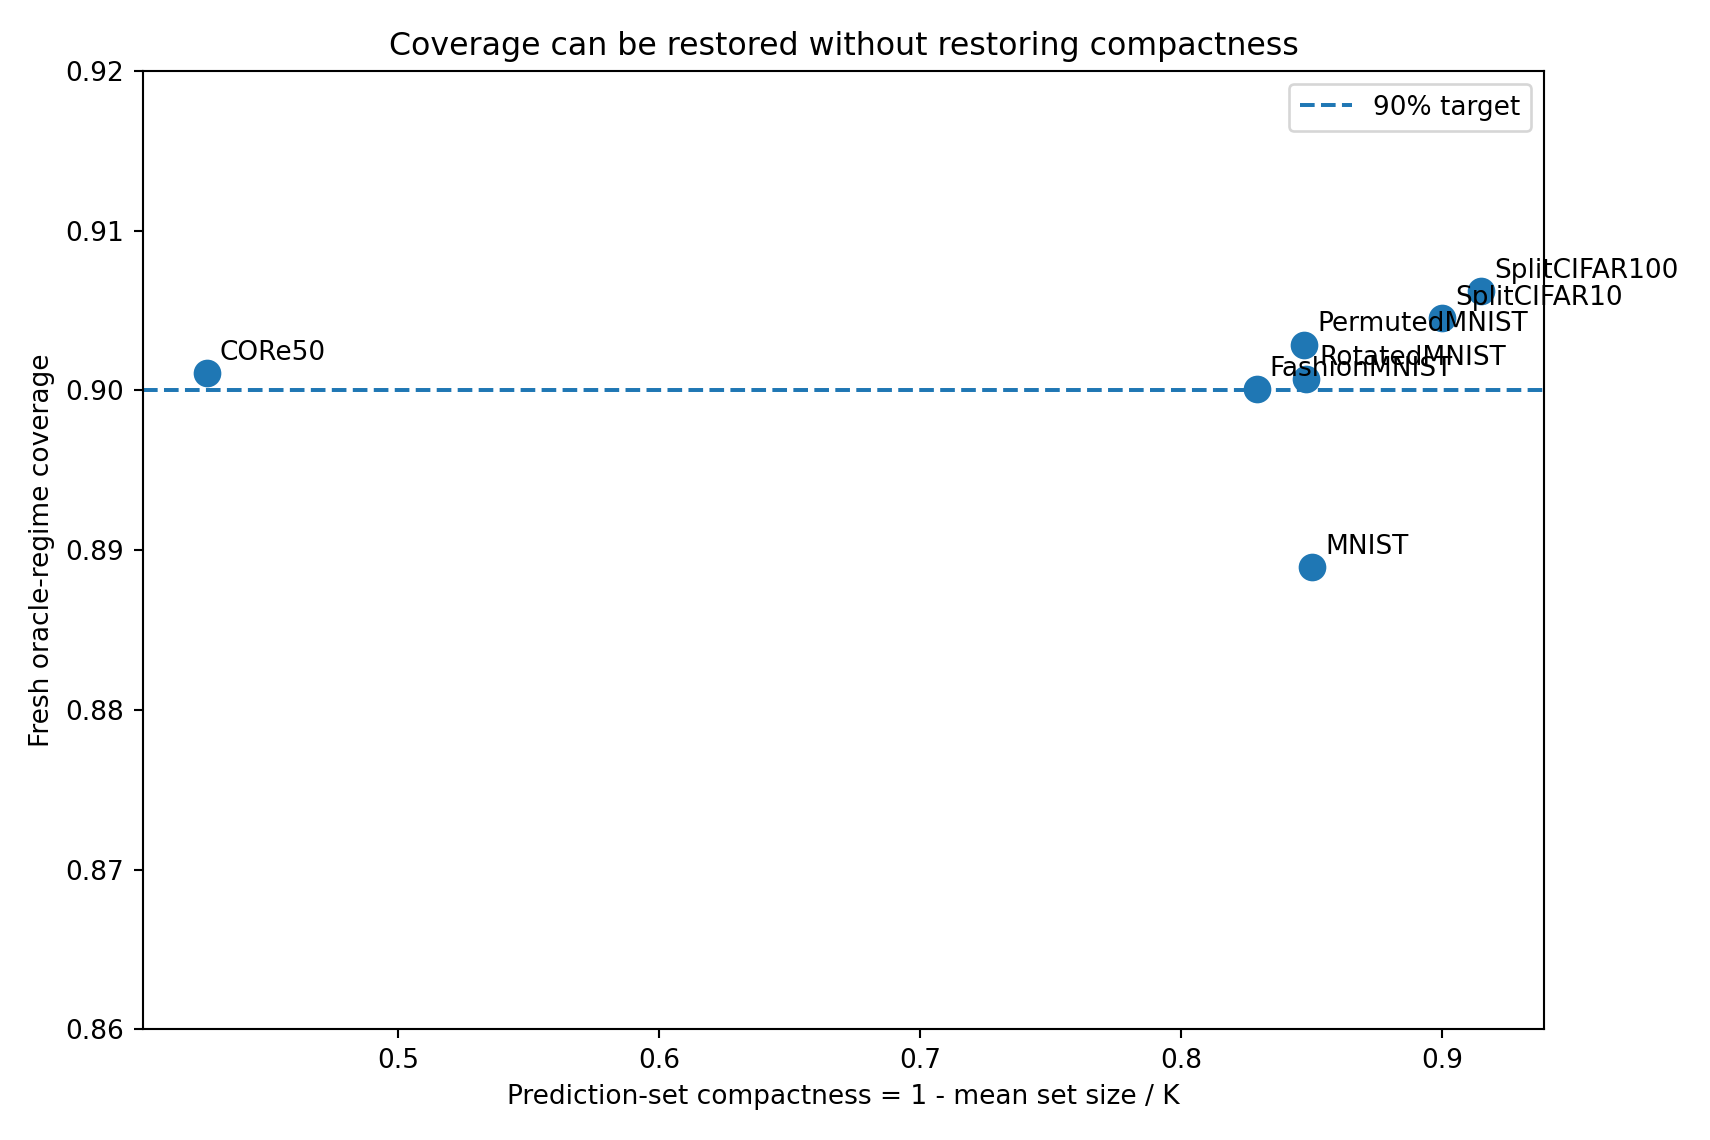
\includegraphics[width=.88\linewidth]{figures/coverage_vs_compactness.png}\caption{Coverage may be restored without restoring compactness.}\end{figure}

\subsection{Global averages hide local failures}
Aggregate coverage can appear acceptable while individual seed-regime cells under-cover severely. Worst-cell reporting is therefore part of the evidence contract, not an optional diagnostic.
\begin{figure}[H]\centering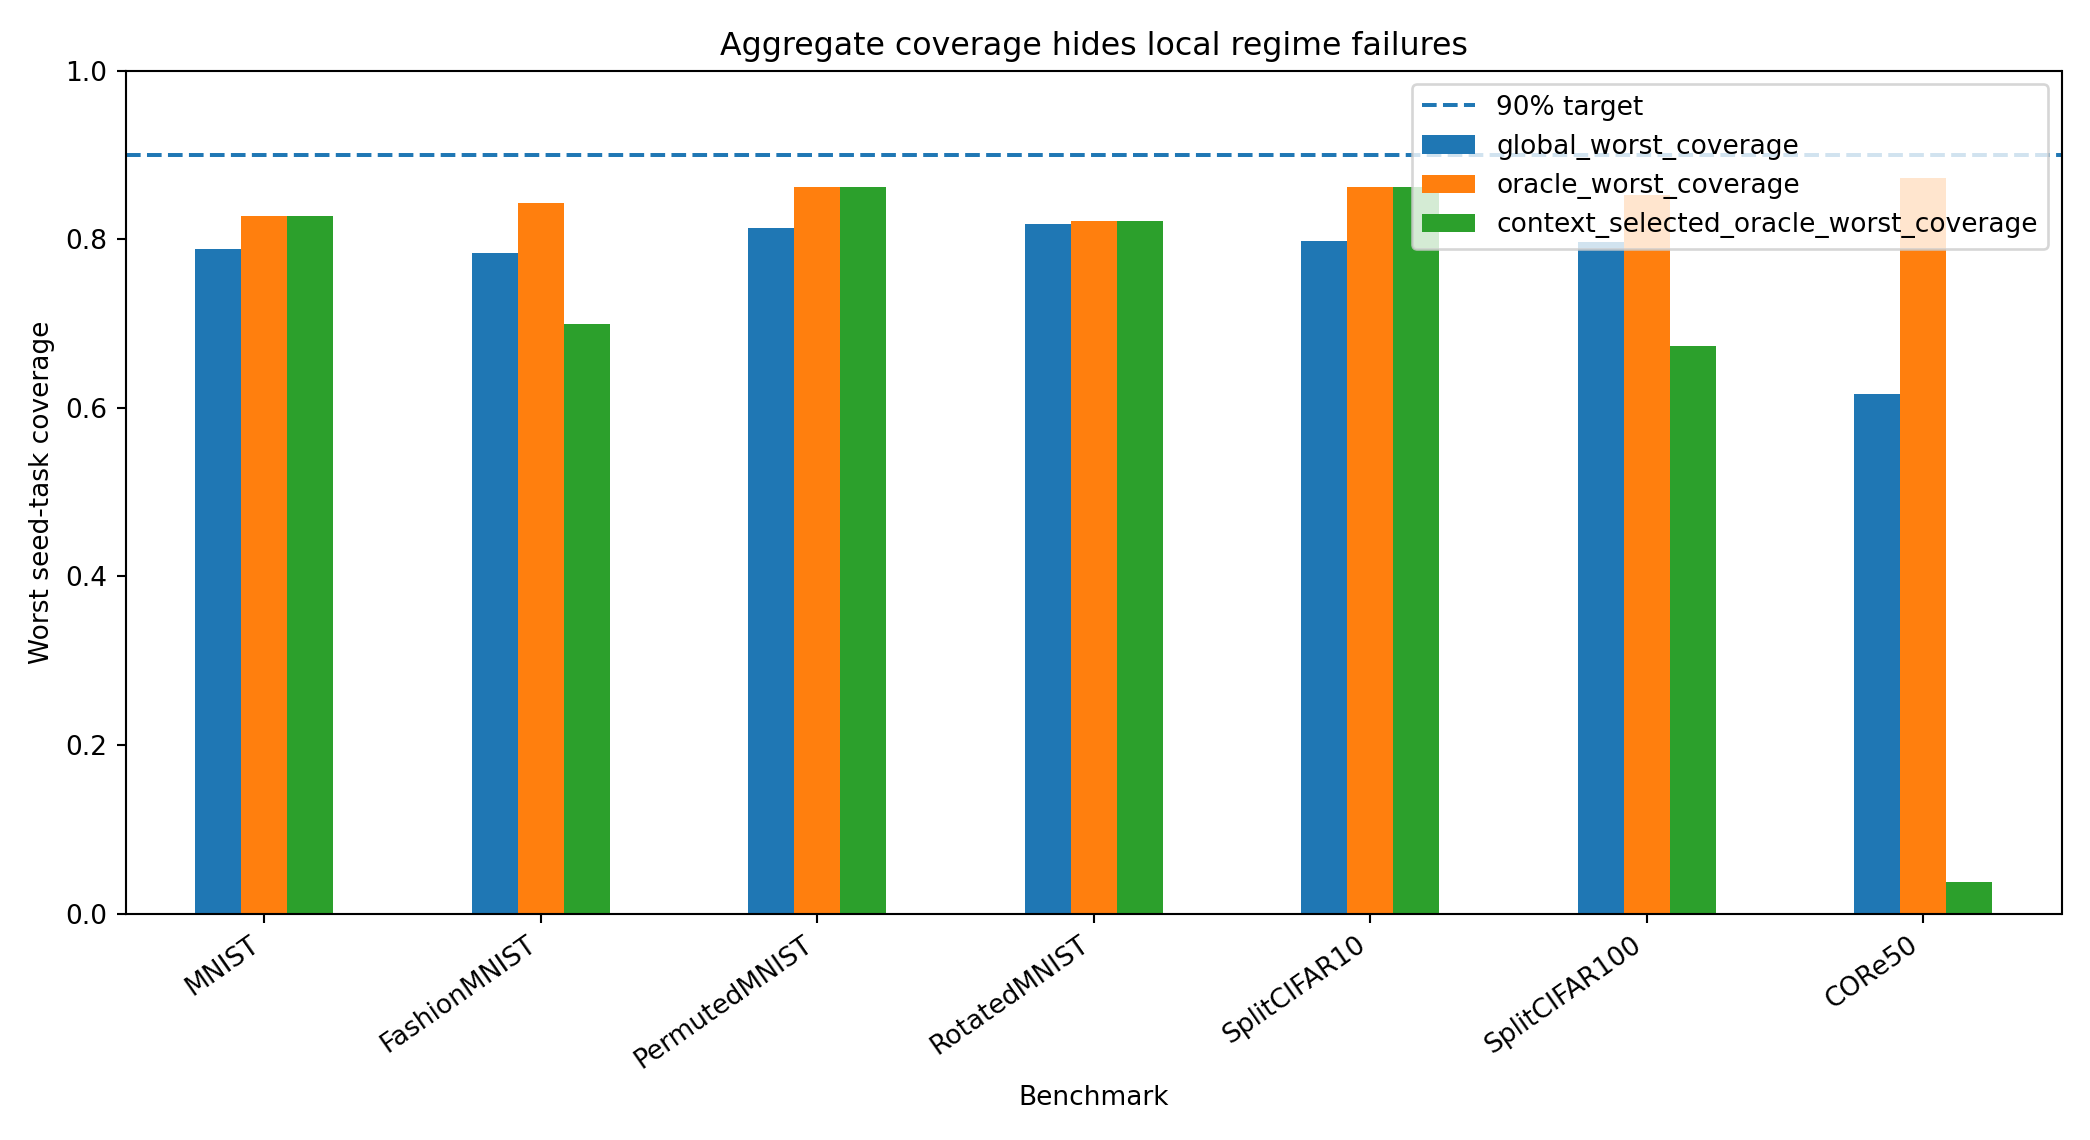
\includegraphics[width=.88\linewidth]{figures/worst_regime_coverage.png}\caption{Worst seed-task coverage under global, fresh oracle, and context-selected oracle calibration.}\end{figure}

\subsection{Stale evidence has two failure modes}
Reusing the T0 quantile causes undercoverage on several MNIST-family runs and SplitCIFAR10. On SplitCIFAR100 and CORe50 it becomes highly conservative, retaining broad sets and little actionability. Staleness is a mismatch, not simply overconfidence.
\begin{figure}[H]\centering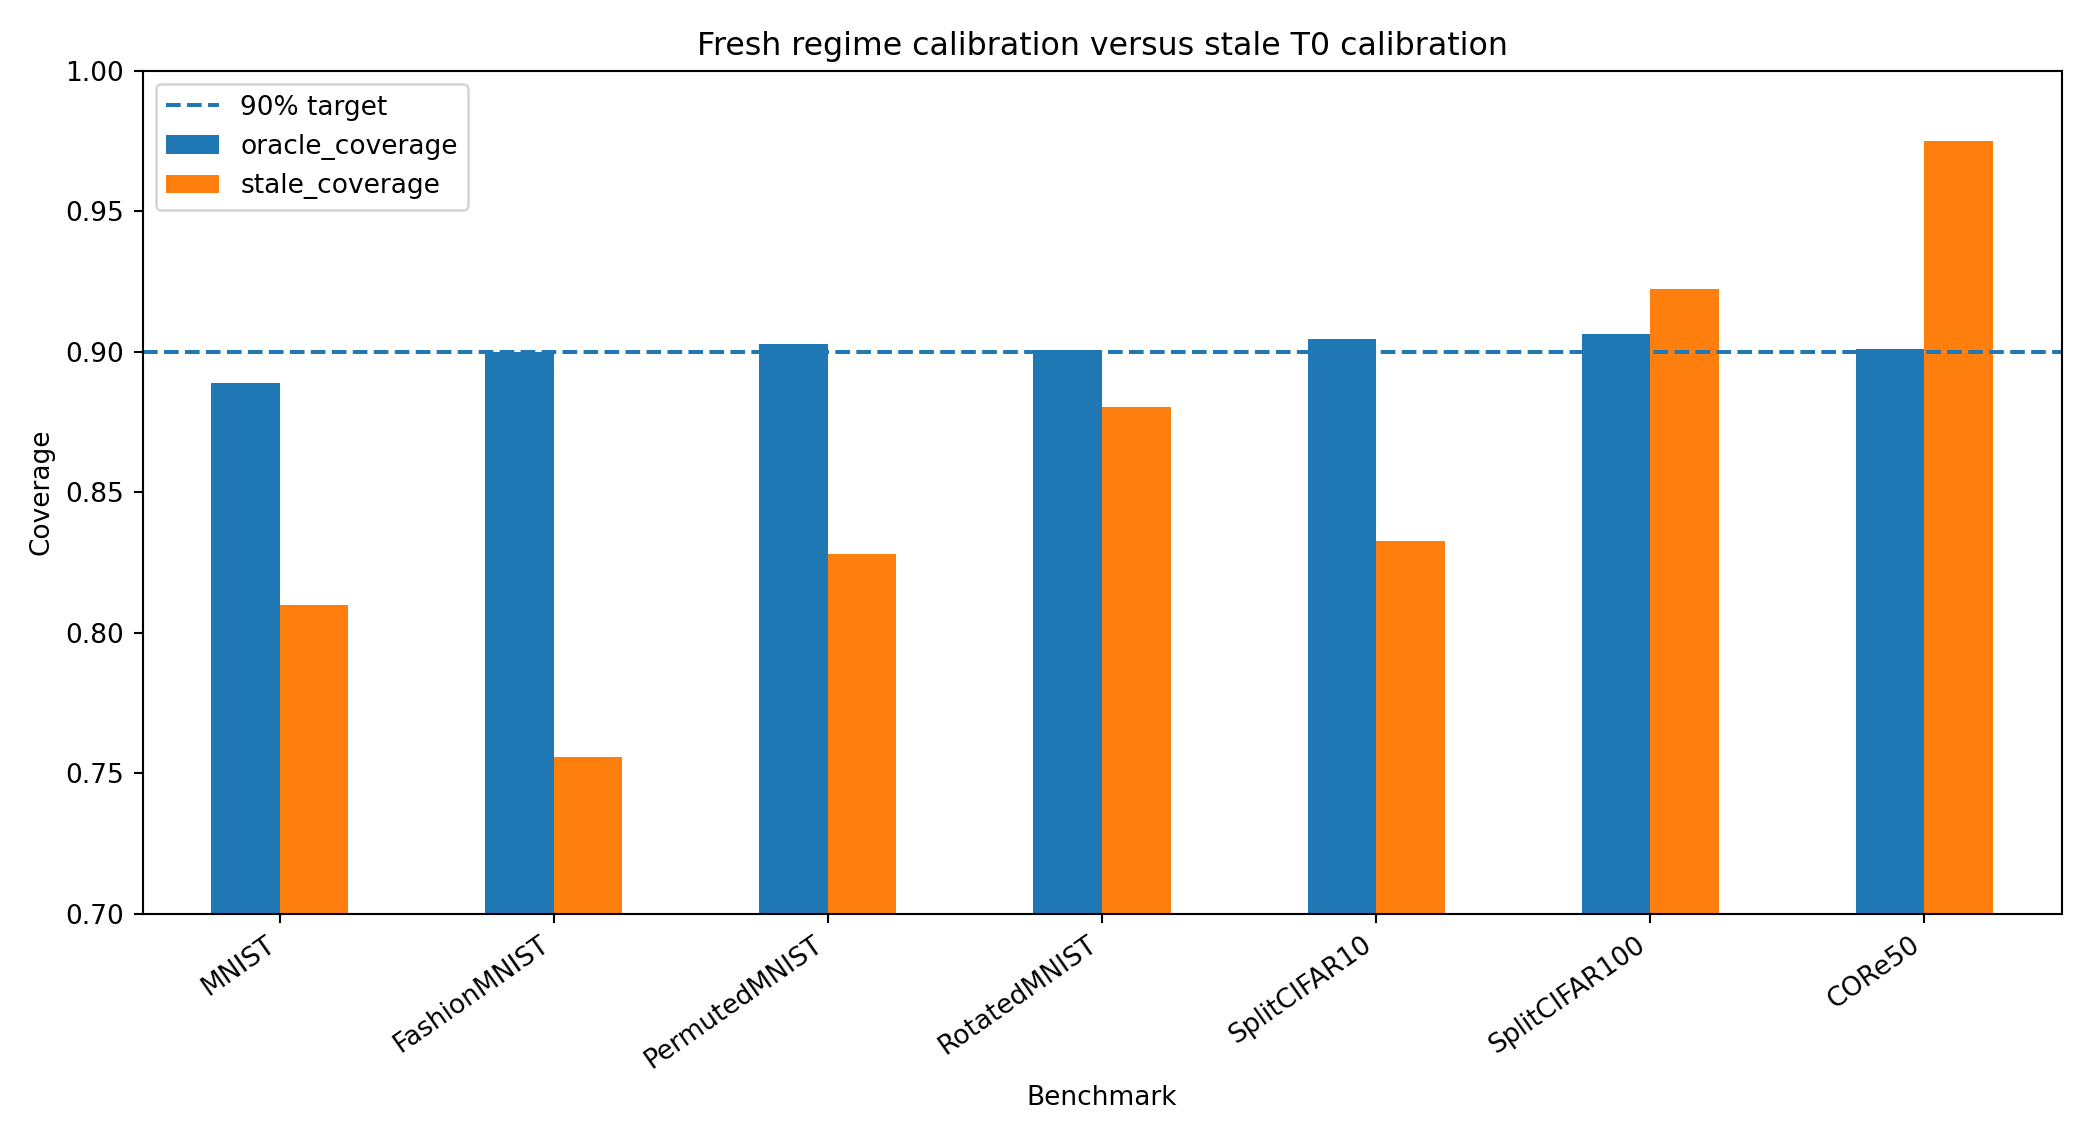
\includegraphics[width=.88\linewidth]{figures/fresh_vs_stale_coverage.png}\caption{Fresh regime calibration versus stale T0 calibration.}\end{figure}

\subsection{Wrong context recalls wrong evidence}
On CORe50, coverage decreases from 0.9011 under fresh oracle-regime calibration to 0.7255 when the same regime-specific calibrators are selected using inferred context, a 17.6 percentage-point loss. A statistically valid calibrator is not safe when recalled for the wrong situation.
\begin{figure}[H]\centering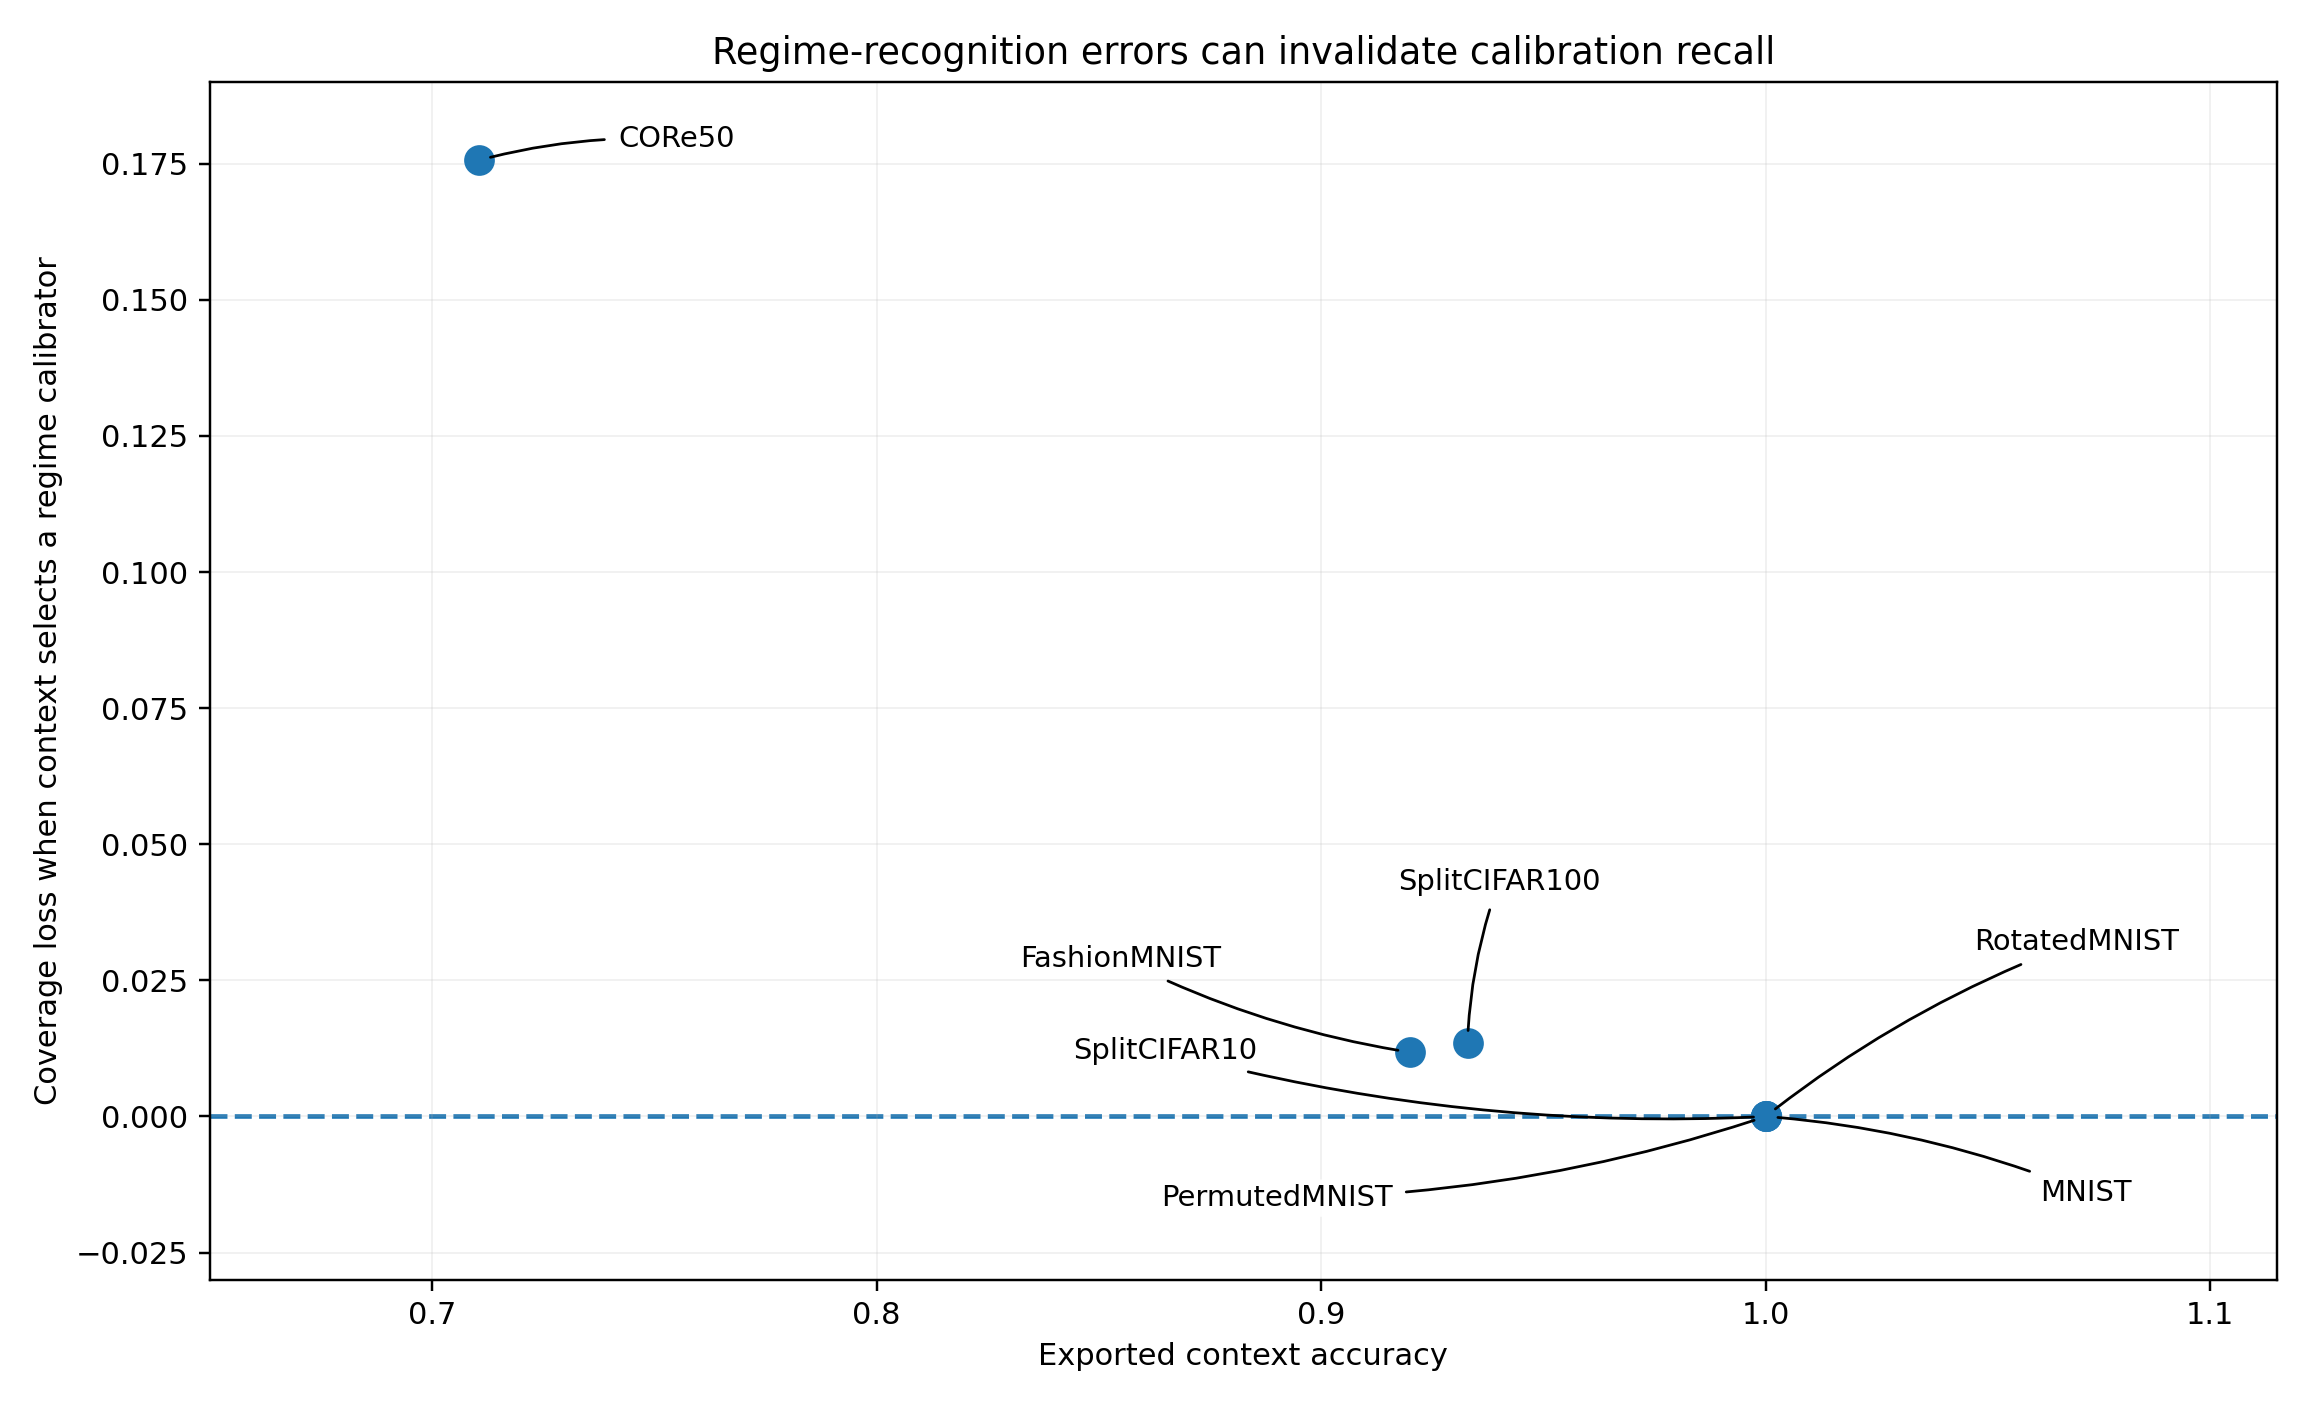
\includegraphics[width=.88\linewidth]{figures/context_accuracy_vs_recall_loss.png}\caption{Context errors translate into calibration-recall loss.}\end{figure}

\section{FashionMNIST RC2O Consistency Patch}
The original v0.3 synthesis used an older RC2M-alpha trace. Version 0.3.1 introduced the RC2O-v1 trace; version 0.3.2 preserves that correction in a fully reproducible release. Final average accuracy rises from 0.8872 to 0.9010, context accuracy from 0.88 to 0.92, mean set size falls from 1.0906 to 1.0269, and singleton action rises from 86.48\% to 89.83\%, while fresh coverage remains approximately 0.90.

\begin{quote}
\textbf{RC2O does not primarily win on coverage---coverage is imposed by calibration---but on predictive competence, context recognition, prediction-set compactness, and action rate.}
\end{quote}

\section{What the Results Say About MMALS-CAL}
The evidence supports five conclusions: fresh calibration repairs coverage rather than competence; valid calibration can be invalidated by wrong regime recall; global coverage can hide local undercoverage; stale evidence can under-cover or become non-actionably conservative; and actionability is separate from coverage.

These conclusions also define what \mmalscal{} is: an empirical and statistical evidence-verification layer that exposes disagreement between learning, regime recognition, uncertainty, and action. It is not a learned replacement for the backbone and not a universal safety proof.

\section{Engineering After the PhD}
A production implementation should remain a fail-closed evidence shell around MMALS. It requires a label-free early-warning detector, delayed-label confirmation, an immutable calibration registry, strict temporal separation of detection/calibration/validation windows, a conformal set builder, a cost-aware gate, and an evidence ledger. The online chain should be
\begin{equation}
\text{detect}\rightarrow\text{close}\rightarrow\text{buffer without leakage}\rightarrow\text{recalibrate}\rightarrow\text{validate}\rightarrow\text{reopen}.
\end{equation}
CUSUM should be an interpretable baseline and BOCPD a probabilistic comparator. TPUT/STRAT-Q may later optimize wrong-action, abstention, evidence, latency, and retention costs while keeping the conformal constraint explicit.

\section{For a 12-Year-Old}
Imagine a puzzle team with different specialists. The MMALS mycelial network helps send each puzzle to useful specialists. MMALS-CAL is the referee. It asks whether the team learned the puzzle, recognized its type, still has a fresh confidence rule, and has one clear answer. The conformal quantile is a line drawn across earlier ``surprise scores.'' Answers that are not more surprising than the line enter a candidate set. One candidate can mean ACTION; several candidates mean ``I am not sure yet.'' Saying ``one of 29 labels'' can be honest but not useful enough to act.

\section{Limitations}
This release is an offline replay of exported final-checkpoint traces. It does not implement online label-free CUSUM or BOCPD, delayed labels, streaming role assignment, live calibration expiry, or automatic gate reopening. Context values are exported by source runs and must still be audited for independence from explicit task identifiers. Coverage is marginal, not conditional for every subgroup or time interval.

SplitCIFAR10, SplitCIFAR100, and CORe50 use frozen small-CNN feature representations. Low actionability may therefore reflect limitations of both the upstream representation and the continual learner; the present paper does not establish backbone sensitivity or invariance. Finally, the singleton gate is a conservative cross-benchmark baseline for autonomous single-label actionability, not a universal deployment policy or the maximum achievable action rate.

\section{Reproducibility}
Unlike v0.3.1, the v0.3.2 GitHub package contains the complete replay code and all seven compressed filtered traces. The original multi-hundred-megabyte evidence packages are not required for numerical reproduction and are omitted from Git. Exact filenames, checksums, and blank user-supplied Drive/archive location fields are provided for future provenance recovery.

\section{Roadmap}
The next stage is \textbf{MMALS-CAL v0.4: Online Regime Freshness and Change-Detection Harness}. It should compare fixed calibration, periodic recalibration, oracle change points, label-free CUSUM, delayed-label CUSUM, BOCPD, and adaptive conformal baselines. Evaluation must include false alarms, detection delay, coverage during transition, contamination, time to restored coverage, ACTION, wrong-action rate, and abstention cost.

\section{Conclusion}
\mmalscal{} adds a missing evidential layer to continual learning. It asks not only whether a system learned, but whether it recognized the situation, whether its uncertainty rule remains valid, whether the resulting set is compact, and whether action is justified. Calibration can control marginal coverage; it cannot manufacture competence, repair a wrong context, or turn a broad set into a useful decision. A trustworthy system must be able to say both ``I can act'' and ``I do not yet have enough fresh evidence.''

\clearpage
\section{Annotated References: Abstracts, Engineer Translations, and Contributions to MMALS-CAL}
Below, \textbf{``abstract'' means a concise paraphrase of the work's contribution}, not a reproduction of the publisher's official abstract.

\subsection{How the references fit together}\label{how-the-references-fit-together}

\begin{longtable}[]{@{}
  >{\raggedright\arraybackslash}p{(\columnwidth - 4\tabcolsep) * \real{0.3333}}
  >{\raggedright\arraybackslash}p{(\columnwidth - 4\tabcolsep) * \real{0.3333}}
  >{\raggedright\arraybackslash}p{(\columnwidth - 4\tabcolsep) * \real{0.3333}}@{}}
\toprule\noalign{}
\begin{minipage}[b]{\linewidth}\raggedright
Role in MMALS-CAL
\end{minipage} & \begin{minipage}[b]{\linewidth}\raggedright
References
\end{minipage} & \begin{minipage}[b]{\linewidth}\raggedright
Status in v0.3.2
\end{minipage} \\
\midrule\noalign{}
\endhead
\bottomrule\noalign{}
\endlastfoot
Foundations of conformal prediction & Vovk et al.; Angelopoulos \& Bates & Directly implemented \\
Coverage versus set compactness & Sadinle et al. & Direct conceptual support \\
Online adaptation under drift & Gibbs \& Candès 2021/2022; Bhatnagar et al. & Roadmap, not yet implemented \\
Automatic regime-change detection & Page; Adams \& MacKay & Roadmap component A \\
Fail-closed and constraint-oriented design & Thomas et al. & Architectural and verification philosophy \\
\end{longtable}

\begin{center}\rule{0.5\linewidth}{0.5pt}\end{center}

\subsection{1. Vovk, Gammerman, and Shafer, 2005}\label{vovk-gammerman-and-shafer-2005}

\subsubsection{\texorpdfstring{\emph{Algorithmic Learning in a Random World}}{Algorithmic Learning in a Random World}}\label{algorithmic-learning-in-a-random-world}

\paragraph{Paraphrased abstract}\label{paraphrased-abstract}

This foundational book develops conformal prediction as a way to attach statistically meaningful confidence information to machine-learning predictions. Instead of returning only a point prediction, a conformal predictor evaluates how unusual---or non-conforming---a candidate output is relative to previously observed examples. Under the classical randomness or exchangeability assumptions, the resulting prediction regions have controlled error rates without requiring the underlying predictive model to be probabilistically correct. The book connects these methods to algorithmic randomness, online prediction, confidence, and credibility. (\href{https://link.springer.com/book/10.1007/b106715?utm_source=chatgpt.com}{link.springer.com})

\paragraph{Engineer translation}\label{engineer-translation}

You already have a classifier producing scores. Conformal prediction adds an external validation wrapper:

\begin{lstlisting}
model scores
    ↓
nonconformity score
    ↓
calibration quantile
    ↓
prediction set with a measurable error rate
\end{lstlisting}

The important engineering idea is that \textbf{the classifier does not need to estimate perfect probabilities}. The calibration layer looks at how the scores behaved on held-out data and converts them into a prediction set.

For MMALS-CAL, this is the origin of:

\[
s(x,y)=1-p(y\mid x)
\]

and:

\[
\Gamma(x)=\{y:s(x,y)\leq\widehat q\}.
\]

\paragraph{What it brings to the MMALS-CAL paper}\label{what-it-brings-to-the-mmals-cal-paper}

This is the principal theoretical foundation for:

\begin{itemize}
\tightlist
\item
  the use of nonconformity scores;
\item
  conformal calibration quantiles;
\item
  prediction sets rather than unconditional single-label answers;
\item
  marginal error control under exchangeability;
\item
  separating the predictor from the uncertainty-verification layer.
\end{itemize}

It supports the claim that MMALS-CAL is \textbf{model-agnostic}: it can wrap MMALS outputs without modifying the MMALS learner.

\paragraph{Important limitation}\label{important-limitation}

The classical validity result depends on calibration and deployment observations being exchangeable. It does not automatically remain valid when the operating regime changes.

That limitation is exactly why MMALS-CAL studies:

\begin{itemize}
\tightlist
\item
  stale calibration;
\item
  global versus regime-specific calibration;
\item
  context-selected calibrators;
\item
  future online change detection.
\end{itemize}

\begin{center}\rule{0.5\linewidth}{0.5pt}\end{center}

\subsection{2. Angelopoulos and Bates, 2021}\label{angelopoulos-and-bates-2021}

\subsubsection{\texorpdfstring{\emph{A Gentle Introduction to Conformal Prediction and Distribution-Free Uncertainty Quantification}}{A Gentle Introduction to Conformal Prediction and Distribution-Free Uncertainty Quantification}}\label{a-gentle-introduction-to-conformal-prediction-and-distribution-free-uncertainty-quantification}

\paragraph{Paraphrased abstract}\label{paraphrased-abstract-1}

This tutorial presents conformal prediction as a practical framework for converting the outputs of arbitrary pretrained models into prediction sets or intervals with explicit finite-sample coverage guarantees. It emphasizes that the method requires very few assumptions about the model or data distribution, while still requiring an appropriate exchangeability relationship between calibration and future observations. The paper provides practical examples, implementation guidance, evaluation methods, and extensions to structured prediction, distribution shift, abstention, and risk control. (\href{https://arxiv.org/abs/2107.07511?utm_source=chatgpt.com}{arxiv.org})

\paragraph{Engineer translation}\label{engineer-translation-1}

This paper is the practical manual for turning conformal prediction into software.

The recipe is:

\begin{enumerate}
\def\labelenumi{\arabic{enumi}.}
\tightlist
\item
  train or obtain a predictive model;
\item
  freeze it;
\item
  reserve a calibration dataset;
\item
  calculate one nonconformity score per calibration observation;
\item
  take a finite-sample corrected quantile;
\item
  use this quantile to form sets on new observations;
\item
  evaluate both coverage and set size.
\end{enumerate}

It says, in effect:

\begin{quote}
Do not redesign your neural network merely to obtain uncertainty estimates. Add a statistically controlled layer around its outputs.
\end{quote}

\paragraph{What it brings to the MMALS-CAL paper}\label{what-it-brings-to-the-mmals-cal-paper-1}

It directly supports the practical implementation choices in v0.3.2:

\begin{itemize}
\tightlist
\item
  black-box wrapping of existing MMALS traces;
\item
  held-out calibration data;
\item
  finite-sample quantile correction;
\item
  90\% target coverage;
\item
  reporting set size alongside coverage;
\item
  abstention and prediction-set evaluation.
\end{itemize}

It is probably the best citation for readers who want to understand \textbf{how MMALS-CAL works operationally} without first reading the deeper theoretical literature.

\paragraph{Important nuance}\label{important-nuance}

``Distribution-free'' does not mean ``valid under every possible deployment shift.''

It means that the method does not require a parametric distribution such as Gaussian noise. Classical validity still relies on exchangeability between calibration and deployment data.

\begin{center}\rule{0.5\linewidth}{0.5pt}\end{center}

\subsection{3. Sadinle, Lei, and Wasserman, 2019}\label{sadinle-lei-and-wasserman-2019}

\subsubsection{\texorpdfstring{\emph{Least Ambiguous Set-Valued Classifiers with Bounded Error Levels}}{Least Ambiguous Set-Valued Classifiers with Bounded Error Levels}}\label{least-ambiguous-set-valued-classifiers-with-bounded-error-levels}

\paragraph{Paraphrased abstract}\label{paraphrased-abstract-2}

The paper considers multiclass classifiers that return a set of plausible labels rather than a single label. It formulates the design problem as satisfying a user-specified coverage or error constraint while minimizing ambiguity, measured through the expected size of the returned label set. It derives optimal classifiers when the true class probabilities are known and proposes estimators with theoretical and finite-sample properties when those probabilities must be estimated. It also examines the possibility of empty prediction sets and practical ways to handle them. (\href{https://arxiv.org/abs/1609.00451?utm_source=chatgpt.com}{arxiv.org})

\paragraph{Engineer translation}\label{engineer-translation-2}

Coverage alone is easy to achieve badly.

A system could always return:

\begin{lstlisting}
{every possible class}
\end{lstlisting}

and obtain almost perfect coverage.

That would be statistically correct but operationally useless.

Sadinle et al.~formalize the real engineering objective:

\begin{lstlisting}
meet the error constraint
while
returning the smallest useful set
\end{lstlisting}

This produces two separate metrics:

\begin{itemize}
\tightlist
\item
  \textbf{validity:} is the true answer usually inside the set?
\item
  \textbf{efficiency or ambiguity:} how many answers are inside the set?
\end{itemize}

\paragraph{What it brings to the MMALS-CAL paper}\label{what-it-brings-to-the-mmals-cal-paper-2}

This paper is the strongest support for the distinction between:

\begin{itemize}
\tightlist
\item
  \textbf{coverage}, and
\item
  \textbf{compactness}.
\end{itemize}

It justifies why MMALS-CAL reports both:

\[
\Pr(Y\in\Gamma(X))
\]

and:

\[
\mathbb E[|\Gamma(X)|].
\]

It is directly relevant to the CORe50 result:

\begin{itemize}
\tightlist
\item
  approximately 90\% coverage;
\item
  average set size of about 28.7 labels out of 50;
\item
  almost no singleton actions.
\end{itemize}

The reference helps us argue that \textbf{coverage without low ambiguity is not enough for actionability}.

\paragraph{Important distinction}\label{important-distinction}

MMALS-CAL does not implement the exact optimization procedure proposed by Sadinle et al.

The paper supports our \textbf{compactness axis and engineering objective}, rather than serving as the exact algorithmic source of the LAC split-conformal method used in v0.3.2.

\begin{center}\rule{0.5\linewidth}{0.5pt}\end{center}

\subsection{4. Gibbs and Candès, 2021}\label{gibbs-and-canduxe8s-2021}

\subsubsection{\texorpdfstring{\emph{Adaptive Conformal Inference Under Distribution Shift}}{Adaptive Conformal Inference Under Distribution Shift}}\label{adaptive-conformal-inference-under-distribution-shift}

\paragraph{Paraphrased abstract}\label{paraphrased-abstract-3}

The paper introduces adaptive conformal inference for online environments where the data-generating distribution changes over time. Instead of using one fixed calibration threshold indefinitely, the method continuously adjusts a parameter controlling prediction-set size according to recent coverage errors. The authors prove long-run coverage-frequency behavior without assuming a stationary or exchangeable sequence and demonstrate robustness under substantial real-world distribution shifts. (\href{https://proceedings.neurips.cc/paper/2021/hash/0d441de75945e5acbc865406fc9a2559-Abstract.html}{proceedings.neurips.cc})

\paragraph{Engineer translation}\label{engineer-translation-3}

Classical split conformal works like a fixed configuration:

\begin{lstlisting}
calibrate once
→ obtain threshold
→ reuse threshold
\end{lstlisting}

Adaptive conformal inference adds a feedback loop:

\begin{lstlisting}
produce prediction set
→ later receive true label
→ check whether coverage failed
→ widen or narrow future sets
\end{lstlisting}

It behaves like a controller:

\begin{itemize}
\tightlist
\item
  too many misses → become more conservative;
\item
  too much excess coverage → potentially tighten the sets.
\end{itemize}

\paragraph{What it brings to the MMALS-CAL paper}\label{what-it-brings-to-the-mmals-cal-paper-3}

This reference supports the transition from:

\begin{quote}
offline evidence verification
\end{quote}

to:

\begin{quote}
online adaptive calibration.
\end{quote}

It is central to the proposed v0.4 roadmap.

It shows that the stale-calibrator problem observed experimentally in MMALS-CAL is not merely descriptive. There is an existing theoretical family of methods designed to update coverage control during changing conditions.

\paragraph{\texorpdfstring{What it does \textbf{not} provide to v0.3.2}{What it does not provide to v0.3.2}}\label{what-it-does-not-provide-to-v0.3.2}

Adaptive conformal inference is not implemented in v0.3.2.

The current release:

\begin{itemize}
\tightlist
\item
  uses offline final-checkpoint traces;
\item
  constructs fixed quantiles from reserved calibration subsets;
\item
  compares fresh and stale quantiles;
\item
  does not update quantiles sequentially.
\end{itemize}

Also, adaptive conformal inference is an adaptation mechanism, not necessarily a semantic detector that announces which named MMALS regime is active.

\begin{center}\rule{0.5\linewidth}{0.5pt}\end{center}

\subsection{5. Gibbs and Candès, 2022}\label{gibbs-and-canduxe8s-2022}

\subsubsection{\texorpdfstring{\emph{Conformal Inference for Online Prediction with Arbitrary Distribution Shifts}}{Conformal Inference for Online Prediction with Arbitrary Distribution Shifts}}\label{conformal-inference-for-online-prediction-with-arbitrary-distribution-shifts}

\paragraph{Paraphrased abstract}\label{paraphrased-abstract-4}

This work extends adaptive conformal inference to respond more effectively to changing environments. It addresses the problem that excessive reliance on historical observations can make an online conformal method react too slowly. The proposed procedure dynamically tunes its adaptation rate and provides regret guarantees over local time intervals, allowing it to respond to distribution shifts of different sizes and speeds without prior knowledge of the shift dynamics. (\href{https://arxiv.org/abs/2208.08401?utm_source=chatgpt.com}{arxiv.org})

\paragraph{Engineer translation}\label{engineer-translation-4}

The 2021 method needs an update speed:

\begin{itemize}
\tightlist
\item
  update too slowly → the system remains stale after a change;
\item
  update too quickly → the threshold becomes noisy and unstable.
\end{itemize}

The 2022 method effectively manages several possible adaptation speeds and learns which one is useful.

Engineer analogy:

\begin{lstlisting}
slow controller  → stable but sluggish
fast controller  → reactive but noisy
adaptive controller → chooses speed from recent behavior
\end{lstlisting}

\paragraph{What it brings to the MMALS-CAL paper}\label{what-it-brings-to-the-mmals-cal-paper-4}

It supports two important observations from our experiments:

\begin{enumerate}
\def\labelenumi{\arabic{enumi}.}
\tightlist
\item
  \textbf{Calibration age matters.}
\item
  \textbf{Not all changes occur at the same speed.}
\end{enumerate}

PermutedMNIST resembles a relatively abrupt functional shift, while RotatedMNIST suggests a more ordered or gradual geometric variation. A fixed adaptation speed may not be appropriate for both.

This paper is therefore relevant to:

\begin{itemize}
\tightlist
\item
  calibration freshness;
\item
  local-window evaluation;
\item
  adaptive recalibration speed;
\item
  the future comparison between fixed, periodic, and adaptive calibration.
\end{itemize}

\paragraph{Important limitation}\label{important-limitation-1}

This reference does not mean that MMALS-CAL v0.3.2 is already robust to arbitrary shifts.

It defines a candidate future method that should be compared against:

\begin{itemize}
\tightlist
\item
  fixed calibration;
\item
  periodic recalibration;
\item
  CUSUM-triggered recalibration;
\item
  oracle change points.
\end{itemize}

\begin{center}\rule{0.5\linewidth}{0.5pt}\end{center}

\subsection{6. Bhatnagar, Wang, Xiong, and Bai, 2023}\label{bhatnagar-wang-xiong-and-bai-2023}

\subsubsection{\texorpdfstring{\emph{Improved Online Conformal Prediction via Strongly Adaptive Online Learning}}{Improved Online Conformal Prediction via Strongly Adaptive Online Learning}}\label{improved-online-conformal-prediction-via-strongly-adaptive-online-learning}

\paragraph{Paraphrased abstract}\label{paraphrased-abstract-5}

The authors study online prediction sets when distributions may change arbitrarily. They argue that performance measured over the entire history can hide failures during shorter local intervals. They introduce strongly adaptive online conformal methods that control regret simultaneously over intervals of different lengths and obtain approximately valid coverage. Their experiments show improved local coverage and smaller prediction sets under distribution shift compared with earlier methods. (\href{https://proceedings.mlr.press/v202/bhatnagar23a.html}{proceedings.mlr.press})

\paragraph{Engineer translation}\label{engineer-translation-5}

Imagine a system that is correct over one year on average but fails badly for two weeks after every regime change.

A global annual metric may still look acceptable.

Strongly adaptive methods ask:

\begin{quote}
Did the system perform correctly on every meaningful local interval?
\end{quote}

The proposed architecture uses multiple online experts, each active over different temporal intervals. This allows the system to adapt to:

\begin{itemize}
\tightlist
\item
  short abrupt shifts;
\item
  long stable periods;
\item
  medium-duration changes;
\end{itemize}

without choosing one fixed monitoring window in advance.

\paragraph{What it brings to the MMALS-CAL paper}\label{what-it-brings-to-the-mmals-cal-paper-5}

This reference strongly supports one of our main findings:

\begin{quote}
Aggregate coverage can conceal local undercoverage.
\end{quote}

MMALS-CAL already reports:

\begin{itemize}
\tightlist
\item
  global coverage;
\item
  seed-level coverage;
\item
  task-level coverage;
\item
  worst seed-task coverage.
\end{itemize}

Bhatnagar et al.~provide a theoretical online continuation of that idea: validity and efficiency should also be monitored over \textbf{local time windows}, not only over the complete run.

This is highly relevant to future metrics such as:

\begin{itemize}
\tightlist
\item
  worst-window coverage;
\item
  local coverage error;
\item
  recovery time after drift;
\item
  window-dependent action rate.
\end{itemize}

\paragraph{Current versus future status}\label{current-versus-future-status}

MMALS-CAL v0.3.2 already adopts the \textbf{evaluation philosophy} of local auditing, but it does not implement SAOCP or strongly adaptive online learning.

\begin{center}\rule{0.5\linewidth}{0.5pt}\end{center}

\subsection{7. Adams and MacKay, 2007}\label{adams-and-mackay-2007}

\subsubsection{\texorpdfstring{\emph{Bayesian Online Changepoint Detection}}{Bayesian Online Changepoint Detection}}\label{bayesian-online-changepoint-detection}

\paragraph{Paraphrased abstract}\label{paraphrased-abstract-6}

This paper presents an online Bayesian method for detecting abrupt changes in the generative mechanism of sequential observations. The method maintains a probability distribution over the current run length---the time elapsed since the most recent changepoint. New observations update the posterior probability of each possible run length, allowing the system to represent both the likely position of a change and uncertainty about that position. (\href{https://arxiv.org/abs/0710.3742?utm_source=chatgpt.com}{arxiv.org})

\paragraph{Engineer translation}\label{engineer-translation-6}

Rather than returning only:

\begin{lstlisting}
change / no change
\end{lstlisting}

BOCPD returns something closer to:

\begin{lstlisting}
70% probability that the current regime began 3 samples ago
20% probability that it began 8 samples ago
10% probability that no recent change occurred
\end{lstlisting}

Its internal state is the posterior distribution:

\[
P(r_t\mid x_{1:t}),
\]

where \(r_t\) is the current run length.

\paragraph{What it brings to the MMALS-CAL paper}\label{what-it-brings-to-the-mmals-cal-paper-6}

It provides the probabilistic design option for component A:

\begin{quote}
automatic regime-change detection.
\end{quote}

BOCPD would allow future MMALS-CAL versions to:

\begin{itemize}
\tightlist
\item
  identify suspected regime transitions;
\item
  quantify uncertainty about the transition;
\item
  estimate how long the current regime has existed;
\item
  decide whether enough post-change observations have accumulated for calibration;
\item
  trigger quarantine and buffer creation.
\end{itemize}

\paragraph{Important limitation}\label{important-limitation-2}

BOCPD requires an explicit probabilistic model for observations and a hazard model for changepoints.

It is not distribution-free in the conformal-prediction sense.

For MMALS-CAL, a design question remains:

\begin{quote}
What signal should BOCPD observe?
\end{quote}

Candidates include:

\begin{itemize}
\tightlist
\item
  prediction entropy;
\item
  context entropy;
\item
  route drift;
\item
  embedding drift;
\item
  delayed-label nonconformity;
\item
  empirical miscoverage.
\end{itemize}

\begin{center}\rule{0.5\linewidth}{0.5pt}\end{center}

\subsection{8. Page, 1954}\label{page-1954}

\subsubsection{\texorpdfstring{\emph{Continuous Inspection Schemes}}{Continuous Inspection Schemes}}\label{continuous-inspection-schemes}

\paragraph{Paraphrased abstract}\label{paraphrased-abstract-7}

Page studies sequential monitoring procedures designed to detect when an observed process has moved away from its expected operating condition. The central idea underlying CUSUM is to accumulate small deviations over time so that a persistent shift becomes detectable even when each individual observation is not sufficiently unusual to trigger an alarm. The method balances detection delay against false alarms through its reference value and alarm threshold. (\href{https://www.jstor.org/stable/2333009?utm_source=chatgpt.com}{jstor.org})

\paragraph{Engineer translation}\label{engineer-translation-7}

A single strange observation may be noise.

Ten slightly strange observations in the same direction may indicate a real regime change.

CUSUM keeps a running statistic such as:

\[
S_t=\max(0,S_{t-1}+z_t-k),
\]

and raises an alarm when:

\[
S_t>h.
\]

Where:

\begin{itemize}
\tightlist
\item
  \(z_t\) is the monitored deviation;
\item
  \(k\) ignores small expected fluctuations;
\item
  \(h\) controls alarm sensitivity.
\end{itemize}

\paragraph{What it brings to the MMALS-CAL paper}\label{what-it-brings-to-the-mmals-cal-paper-7}

CUSUM is the simplest interpretable candidate for component A.

It is attractive because it is:

\begin{itemize}
\tightlist
\item
  incremental;
\item
  computationally cheap;
\item
  easy to audit;
\item
  suitable for real-time systems;
\item
  explicit about the false-alarm versus detection-delay trade-off.
\end{itemize}

For MMALS-CAL, it could monitor separate channels:

\begin{lstlisting}
CUSUM on class uncertainty
CUSUM on context uncertainty
CUSUM on route drift
CUSUM on embedding drift
CUSUM on delayed-label nonconformity
\end{lstlisting}

\paragraph{Important limitation}\label{important-limitation-3}

CUSUM detects sustained change in a chosen signal. It does not explain the semantic meaning of the new regime, and it is only as good as:

\begin{itemize}
\tightlist
\item
  the monitored statistic;
\item
  the reference distribution;
\item
  the selected threshold;
\item
  the assumed shift direction.
\end{itemize}

It should therefore not be confused with MMALS context inference itself.

\begin{center}\rule{0.5\linewidth}{0.5pt}\end{center}

\subsection{9. Thomas et al., 2019}\label{thomas-et-al.-2019}

\subsubsection{\texorpdfstring{\emph{Preventing Undesirable Behavior of Intelligent Machines}}{Preventing Undesirable Behavior of Intelligent Machines}}\label{preventing-undesirable-behavior-of-intelligent-machines}

\paragraph{Paraphrased abstract}\label{paraphrased-abstract-8}

The paper proposes a framework for designing machine-learning algorithms around explicit user-defined constraints on undesirable behavior. Rather than expecting users to indirectly control risk through penalties or hyperparameters, the framework asks them to specify the behavior that must be avoided and the acceptable probability of violation. The resulting Seldonian approach may refuse to return a solution when the available evidence is insufficient to support the required constraint. The authors demonstrate the approach on examples involving harmful or unfair behavior. (\href{https://www.science.org/doi/10.1126/science.aag3311?utm_source=chatgpt.com}{science.org})

\paragraph{Engineer translation}\label{engineer-translation-8}

Normal ML design asks:

\begin{quote}
Which model maximizes performance?
\end{quote}

The Seldonian design question is:

\begin{quote}
Which model maximizes performance while giving us enough statistical evidence that an undesirable condition will not be violated?
\end{quote}

And when evidence is insufficient:

\begin{lstlisting}
do not return a supposedly safe solution
\end{lstlisting}

This is the same general fail-closed philosophy as:

\begin{lstlisting}
insufficient evidence
→ NO_DECISION
\end{lstlisting}

\paragraph{What it brings to the MMALS-CAL paper}\label{what-it-brings-to-the-mmals-cal-paper-8}

This reference supports the \textbf{system-design philosophy}, especially:

\begin{itemize}
\tightlist
\item
  explicit undesirable outcomes;
\item
  evidence-based constraints;
\item
  separating candidate construction from independent verification;
\item
  refusing to act when the constraint cannot be supported;
\item
  moving responsibility from the end user to the algorithm and protocol designer.
\end{itemize}

It also connects strongly to the MMALS Verification Stack:

\begin{lstlisting}
candidate result
    ↓
protocol verification
    ↓
statistical safety/evidence test
    ↓
release, ACTION, or refusal
\end{lstlisting}

\paragraph{Critical distinction}\label{critical-distinction}

MMALS-CAL is \textbf{not currently a Seldonian algorithm}.

The guarantee types differ:

\begin{itemize}
\tightlist
\item
  conformal prediction controls marginal coverage of prediction sets;
\item
  Seldonian methods seek high-probability satisfaction of explicitly specified behavioral constraints.
\end{itemize}

Thomas et al.~support our \textbf{fail-closed architecture and claim discipline}, but they should not be cited as proof that MMALS-CAL provides broad machine-safety guarantees.

\begin{center}\rule{0.5\linewidth}{0.5pt}\end{center}

\subsection{What the references collectively bring to MMALS-CAL}\label{what-the-references-collectively-bring-to-mmals-cal}

\subsubsection{1. They establish the statistical foundation}\label{they-establish-the-statistical-foundation}

Vovk et al.~and Angelopoulos--Bates justify the transformation:

\begin{lstlisting}
model output
→ calibrated prediction set
→ measurable marginal coverage
\end{lstlisting}

Without these references, MMALS-CAL could look like an ad hoc confidence-thresholding mechanism.

With them, it is situated within conformal prediction.

\subsubsection{2. They justify the five-axis decomposition}\label{they-justify-the-five-axis-decomposition}

Sadinle et al.~show why coverage must be separated from ambiguity.

That directly supports:

\begin{lstlisting}
Competence
Coverage
Compactness
Context
ACTION
\end{lstlisting}

A system can satisfy coverage while being non-actionable because its sets are too large.

\subsubsection{3. They explain why v0.3.2 is deliberately offline}\label{they-explain-why-v0.3.2-is-deliberately-offline}

Classical split conformal gives the cleanest experimental foundation under controlled calibration/deployment separation.

The online papers demonstrate that the next step is possible, but also that it introduces new questions:

\begin{itemize}
\tightlist
\item
  adaptation rate;
\item
  local-window validity;
\item
  delayed labels;
\item
  temporal dependence;
\item
  calibration recovery;
\item
  shift speed.
\end{itemize}

Thus, v0.3.2 validates components B, C, and a simplified D before adding component A.

\subsubsection{4. They provide two different ways to handle changing regimes}\label{they-provide-two-different-ways-to-handle-changing-regimes}

\paragraph{Explicit change detection}\label{explicit-change-detection}

\begin{itemize}
\tightlist
\item
  Page: lightweight cumulative alarm;
\item
  Adams--MacKay: probabilistic run-length inference.
\end{itemize}

\paragraph{Continuous calibration adaptation}\label{continuous-calibration-adaptation}

\begin{itemize}
\tightlist
\item
  Gibbs--Candès: feedback adaptation;
\item
  FACI-style adaptation to shift speed;
\item
  Bhatnagar et al.: interval-local strongly adaptive methods.
\end{itemize}

These are complementary rather than identical:

\begin{lstlisting}
change detection asks:
“Did the regime change?”

adaptive conformal asks:
“How should the prediction-set threshold evolve?”
\end{lstlisting}

A complete runtime MMALS-CAL may eventually need both.

\subsubsection{5. They justify fail-closed behavior}\label{they-justify-fail-closed-behavior}

Thomas et al.~support the principle that an intelligent system should be allowed to return:

\begin{lstlisting}
insufficient evidence
\end{lstlisting}

rather than being forced to provide an answer.

This gives stronger intellectual grounding to:

\begin{lstlisting}
ACTION / NO_DECISION
\end{lstlisting}

and to MMALS-CAL's prohibited-claims discipline.

\begin{center}\rule{0.5\linewidth}{0.5pt}\end{center}

\subsection{Recommended citation placement in the paper}\label{recommended-citation-placement-in-the-paper}

\begin{longtable}[]{@{}
  >{\raggedright\arraybackslash}p{(\columnwidth - 2\tabcolsep) * \real{0.5000}}
  >{\raggedright\arraybackslash}p{(\columnwidth - 2\tabcolsep) * \real{0.5000}}@{}}
\toprule\noalign{}
\begin{minipage}[b]{\linewidth}\raggedright
Paper section
\end{minipage} & \begin{minipage}[b]{\linewidth}\raggedright
References
\end{minipage} \\
\midrule\noalign{}
\endhead
\bottomrule\noalign{}
\endlastfoot
Introduction to conformal prediction & Vovk et al.; Angelopoulos \& Bates \\
Calibration quantile and exchangeability & Vovk et al.; Angelopoulos \& Bates \\
Coverage versus compactness & Sadinle et al. \\
Stale evidence and distribution shift & Gibbs \& Candès 2021 \\
Future adaptive calibration & Gibbs \& Candès 2021, 2022; Bhatnagar et al. \\
Regime-change detector roadmap & Page; Adams \& MacKay \\
ACTION/NO\_DECISION and fail-closed design & Thomas et al. \\
Limitations & All online references, explicitly marked as not implemented \\
\end{longtable}

\subsubsection{Suggested literature-positioning paragraph}\label{suggested-literature-positioning-paragraph}

MMALS-CAL builds on three complementary research traditions. Classical conformal prediction provides the statistical foundation for converting black-box model scores into prediction sets with finite-sample marginal coverage under exchangeability. Set-valued classification further establishes that coverage alone is insufficient and that ambiguity, measured through prediction-set size, must be controlled separately. Online conformal inference and changepoint-detection methods provide the foundations for the future transition from offline replay to runtime calibration freshness, while Seldonian algorithm design motivates the fail-closed principle that a system should refuse to act when the available evidence cannot support its declared constraint.

The current v0.3.2 release implements offline no-leakage calibration, regime-aware conformal quantiles, compactness auditing, and a conservative singleton ACTION/NO\_DECISION baseline. It does not yet implement CUSUM, Bayesian online changepoint detection, adaptive conformal inference, FACI, or strongly adaptive online conformal prediction. These references therefore serve both as foundations for the implemented verification layer and as explicit methodological anchors for the next online stage.

The most important message is that the bibliography is not one undifferentiated list. It describes the evolution of the project:

\[
\begin{aligned}
&\text{offline conformal validity}\\
&\rightarrow\ \text{compactness and actionability}\\
&\rightarrow\ \text{regime-change detection}\\
&\rightarrow\ \text{online adaptive calibration}\\
&\rightarrow\ \text{fail-closed operational control}.
\end{aligned}
\]


\begin{thebibliography}{99}
\bibitem{vovk2005} V. Vovk, A. Gammerman, and G. Shafer. \emph{Algorithmic Learning in a Random World}. Springer, 2005.
\bibitem{angelopoulos2021} A. Angelopoulos and S. Bates. A gentle introduction to conformal prediction and distribution-free uncertainty quantification. arXiv:2107.07511, 2021.
\bibitem{sadinle2019} M. Sadinle, J. Lei, and L. Wasserman. Least ambiguous set-valued classifiers with bounded error levels. JASA, 2019.
\bibitem{gibbs2021} I. Gibbs and E. Candes. Adaptive conformal inference under distribution shift. NeurIPS, 2021.
\bibitem{gibbs2022} I. Gibbs and E. Candes. Conformal inference for online prediction with arbitrary distribution shifts. arXiv:2208.08401, 2022.
\bibitem{bhatnagar2023} A. Bhatnagar et al. Improved online conformal prediction via strongly adaptive online learning. ICML, 2023.
\bibitem{adams2007} R. Adams and D. MacKay. Bayesian online changepoint detection. arXiv:0710.3742, 2007.
\bibitem{page1954} E. Page. Continuous inspection schemes. Biometrika, 1954.
\bibitem{thomas2019} P. Thomas et al. Preventing undesirable behavior of intelligent machines. Science, 2019.
\end{thebibliography}
\end{document}
